\documentclass[14pt, a4paper]{extarticle}

\usepackage{graphics}
\usepackage[utf8]{inputenc}
\usepackage[T1]{fontenc}
\usepackage{times}
\usepackage[left=2cm, top=2.5cm, text={17cm, 24cm}]{geometry}
\usepackage[czech]{babel}
\usepackage{textcomp}
\usepackage{tipa}

\begin{document}
\begin{titlepage}
\begin{center}
\textsc{\LARGE Vysoké učení technické v~Brně \\ 
\Large Fakulta informačních technologií} \\
\vspace{\stretch{0.200}}
\begin{figure}[h]
\center
{
\includegraphics{FIT_barevne_CMYK_CZ.eps}
}
\end{figure}
\vspace{\stretch{0.182}}
\Large{Dokumentácia k~projektu do predmetov IFJ a~IAL \\}
\Large{\textbf{Implementácia prekladača jazyka IFJ17} \\}
\medskip
\large{Tým 045, varianta I}
\end{center}
\vfill
\noindent 
\large{Peter Grofčík, xgrofc00 (vedúci) 35\% \\
Martin Fujaček, xfujac00 30\% \\
Patrik Krajč, xkrajc17 35\% \\
Rastislav Pôbiš, xpobis00 0\% \\}

\end{titlepage}

\tableofcontents
\clearpage

\section{Práce v~tíme}
 Zo začiatku sme výber častí nechali v~rámci tímu viac-menej voľný a~každý si mohol vybrať časť, ktorú by mohol zvládnuť sám, pričom postupne sa úlohy menili, či inak rozdeľovali. Vedúci tímu Peter Grofčík sa venoval prevažne generátoru kódu, pričom sa podieľal aj na tabuľke symbolov. Martin Fujaček pracoval na tabuľke symbolov, dokumentácii a~z~prevažnej časti sa venoval precedenčnej syntaktickej analýze spolu s~Rastislavom Pôbišom, ktorý sa staral aj o testovanie. Patrik Krajč začal s~implementáciou lexikálneho a~syntaktického analyzátora. Na sémantike pracovali ako Patrik Krajč, tak Peter Grofčík. V~záverečných fázach sa práce na jednotlivých moduloch prelýnali a~každý sa snažil vyriešiť určitý problém bez ohľadu na to, v~ktorej časti sa nachádzal. Pri implementácii sme využili aj moduly pre prácu s~reťazcami a~inštrukčnou páskou, ktoré sú súčasťou jednoduchého demonstračného prekladača.


\section{Lexikálny analyzátor}
Lexikálny analyzátor je založený na deterministickom konečnom automate, ktorý je uvedený na obrázku \ref{scanner}. Jeho úlohou je rozpoznať jednotlivé lexémy zdrojového kódu a~reprezentovať ich ako tokeny. Lexikálny analyzátor je volaný zo syntaktického analyzátora, ktorý ho požiada o~ďalšiu lexému. Obsahuje definície jednotlivých stavov konečného automatu, rovnako aj kľúčových a rezervovaných kľúčových slov jazyka IFJ17 založenom na jazyku FreeBASIC.
Obrázok konečného automatu sa nachádza na poslednej strane.(\pageref{scanner})


\section{Syntaktická analýza}

\subsection{Syntaktický analyzátor}

Vstupným bodom nášho prekladača je syntaktický analyzátor, ktorý sme sa rozhodli implementovať metódou rekurzívneho zostupu. Vyhodnocuje prichádzajúce lexémy na základe syntaktických pravidiel, ktoré sú definované LL gramatikou (viď kapitolu \ref{gram}). Popri syntaktických vykonáva súčasne aj sémantické kontroly. Výrazy sú spracovávané v osobitnom module popísanom nižšie. Až po úspešnom ukončení syntaktickej a~sémantickej kontroly sa volá generátor cieľového kódu. 

\subsection{Precedenčná syntaktická analýza pre výrazy}

Syntax výrazov sa vyhodnocuje podľa zadania na základe precedenčnej tabuľky. Tá je v skutočnosti implementovaná ako menšia tabuľka, než je uvedené v tabuľke \ref{psa}, keďže niektoré stĺpce sú rovnaké ako iné. Preto každý token mapujeme do tabuľky veľkosti $8\times8$, kde sú len prvky \textit{Operátor 1} (operátory + a~-), \textit{Operátor 2} (operátory * a~/), \textit{Operátor 3} (operátor \textbackslash), \textit{(}, \textit{)}, \textit{Relačné operátory} (=, <>, <, <=, >, >=), \textit{i} (identifikátory, typy integer, double, string) a~nakoniec \textit{\$}, (špeciálny ukončovací znak). Prichádzajúce tokeny, rovnako ako tokeny najbližšie vrcholu na pracovnom zásobníku precedenčnej analýzy, sú mapované do tabuľky funkciou \texttt{group\_tokens()}, ktorá podľa zadaného parametru vráti správny index do zmenšenej tabuľky pre konkrétny token. Vstupný reťazec, ktorý analyzujeme v precedenčnej analýze, posiela syntaktický analyzátor v~jednosmernom zozname ako prvý parameter vstupnej funkcie \texttt{psa()}. Tento zoznam obsahuje stringy jednotlivých tokenov, ich typ a~samozrejme ukazovateľ na nasledujúci token v zozname. Ďalšími parametrami sú typ príkazu, v~ktorom sa výraz nachádza (napr. priraďovací, návrat z~funkcie, cyklus ...), názov premennej (ak sa jedná o~priraďovací príkaz, v~opačnom prípade voláme s~NULL) a~názvom funkcie, v~ktorej sa práve nachádza. Tieto informácie sú potrebné pre naplnenie inštrukčnej pásky správnymi inštrukciami.  \\

\bigskip

\begin{table}[h]
\centering
\resizebox{\columnwidth}{!}{
\begin{tabular}{|c|c|c|c|c|c|c|c|c|c|c|c|c|c|c|c|c|c|c|}
\hline
&+&-&*&/&\textbackslash&(&)&=&<>&<&<=&>&>=&id&int&double&string&\$ \\ \hline \hline
+&>&>&<&<&<&<&>&>&>&>&>&>&>&<&<&<&<&> \\ \hline
-&>&>&<&<&<&<&>&>&>&>&>&>&>&<&<&<&<&> \\ \hline
*&>&>&>&>&>&<&>&<&<&<&<&<&<&>&>&>&>&> \\ \hline
/&>&>&>&>&>&<&>&<&<&<&<&<&<&>&>&>&>&> \\ \hline
\textbackslash&>&>&<&<&>&<&>&>&>&>&>&>&>&<&<&<&<&> \\ \hline
(&<&<&<&<&<&<&=&<&<&<&<&<&<&<&<&<&<& \\ \hline
)&>&>&>&>&>&&>&>&>&>&>&>&>&&&&&> \\ \hline
=&<&<&<&<&<&<&>&>&>&>&>&>&>&<&<&<&<&> \\ \hline
<>&<&<&<&<&<&<&>&>&>&>&>&>&>&<&<&<&<&> \\ \hline
<&<&<&<&<&<&<&>&>&>&>&>&>&>&<&<&<&<&> \\ \hline
<=&<&<&<&<&<&<&>&>&>&>&>&>&>&<&<&<&<&> \\ \hline
>&<&<&<&<&<&<&>&>&>&>&>&>&>&<&<&<&<&> \\ \hline
>=&<&<&<&<&<&<&>&>&>&>&>&>&>&<&<&<&<&> \\ \hline
id&>&>&>&>&>&&>&>&>&>&>&>&>&&&&&> \\ \hline 
int&>&>&>&>&>&&>&>&>&>&>&>&>&&&&&> \\ \hline 
double&>&>&>&>&>&&>&>&>&>&>&>&>&&&&&> \\ \hline 
string&>&>&>&>&>&&>&>&>&>&>&>&>&&&&&> \\ \hline 
\$&<&<&<&<&<&<&&<&<&<&<&<&<&<&<&<&<&1 \\ \hline
\end{tabular}
}
\caption{Tabuľka pre precedenčnú analýzu}
\label{psa}
\end{table}


\section{Generátor kódu }
Generátor kódu sa volá po úspešnom ukončení syntaktickej a sémantickej analýzy. Spracúva inštrukčnú pásku a~postupne na štandartný výstup tlačí postupnosť inštrukcií, ktoré sa budú interpretovať. Pri implementácii sme využili modul pre prácu s~inštrukčnou páskou z~jednoduchého demonstračného prekladača, ktorú sme si pre svoje potreby upravili podľa nutnosti.
Pomocné tmp premenné pre výsledky porovnaní si generátor rieši sám keďže je jednoznačné že finálne precedenčkou upravený výraz sa pri porovnaniach skladá z dvoch operandov a operátora. Názvy skokov pre interpret IFJ17 sú tvorené názvami operátorov, typu porovnania a samozrejme čísla poradia tmp premennej, ktorá je pri výraze porovnávaná, aby nedošlo k duplicite v prípade rovnakých výrazov.
\section{Tabuľka symbolov}
Tabuľku symbolov sme implementovali ako binárny vyhľadávací strom podľa postupov preberaných v~predmete IAL. Tabuľka obsahuje odkazy na binárne stromy pre každú funkciu v~programe. Každý uzol obsahuje niekoľko prvkov. Kľúčom, podľa ktorého sa vyhľadáva, je samotný názov premennej resp. funkcie, ktorý je poľom znakov \texttt{name}. Ďalej obsahuje celočíselnú hodnotu \texttt{type}, ktorá určuje dátový typ položky. Nesmú chýbať ukazovatele na ľavý, resp. pravý podstrom \texttt{LPtr} a~\texttt{RPtr}, a tiež ukazatele na parametre funkcií, samozrejme s typom daného parametru.

\section{LL Gramatika}
\label{gram}
\noindent(1) PROG $\rightarrow$ DECFLIST  DEFFLIST  scope  STLIST  end  scope \\
\\
(2) DECFLIST $\rightarrow$ \textepsilon \\
(3) DECFLIST $\rightarrow$ declare  FUN  DECFLIST \\
\\
(4) FUN $\rightarrow$ function  funid  ( PARLIST )  as  TYPE \textit{EOL} \\
\\
(5) DEFFLIST $\rightarrow$ \textepsilon \\
(6) DEFFLIST $\rightarrow$ FUN  STLIST  end  function \textit{EOL} DEFFLIST \\
\\
(7) PARLIST $\rightarrow$ \textepsilon \\
(8) PARLIST $\rightarrow$ id  as  TYPE  PARLIST1 \\
\\
(9) PARLIST1 $\rightarrow$ \textepsilon \\
(10) PARLIST1 $\rightarrow$ ,  id  as  TYPE  PARLIST1 \\
\\
(11) STLIST $\rightarrow$ \textepsilon \\
(12) STLIST $\rightarrow$ STAT \textit{EOL} STLIST \\
\\
(13) STAT $\rightarrow$ \textepsilon \\
(14) STAT $\rightarrow$ DECV \\
(15) STAT $\rightarrow$ DECV = RVALUE \\
(16) STAT $\rightarrow$ id = RVALUE \\
(17) STAT $\rightarrow$ input  id \\
(18) STAT $\rightarrow$ print  E ; PRINT1 \\
(19) STAT $\rightarrow$ if  E  then \textit{EOL} STLIST  else \textit{EOL} STLIST  end  if \\
(20) STAT $\rightarrow$ do  while  E \textit{EOL} STLIST  loop \\
(21) STAT $\rightarrow$ return  E \\
\\
(22) PRINT1 $\rightarrow$ E ; PRINT1 \\
(23) PRINT1 $\rightarrow$ \textepsilon \\
\\
(24) RVALUE $\rightarrow$ E \\
(25) RVALUE $\rightarrow$ funid ( TERMLIST ) \\
\\
(26) DECV $\rightarrow$ dim  id  as  TYPE \\
\\
(27) TYPE $\rightarrow$ integer \\
(28) TYPE $\rightarrow$ double \\
(29) TYPE $\rightarrow$ string \\
\\
(30) TERMLIST $\rightarrow$ \textepsilon \\
(31) TERMLIST $\rightarrow$ TERM , TERMLIST \\
\\
(32) TERM $\rightarrow$ \textepsilon \\
(33) TERM $\rightarrow$ TYPE \\
(34) TERM $\rightarrow$ id \\
\\
E $\rightarrow$ ( E ) \\
E $\rightarrow$ E * E \\
E $\rightarrow$ E / E \\
E $\rightarrow$ E \textbackslash E \\
E $\rightarrow$ E + E \\
E $\rightarrow$ E - E \\
E $\rightarrow$ E = E \\
E $\rightarrow$ E <> E \\
E $\rightarrow$ E < E \\
E $\rightarrow$ E <= E \\
E $\rightarrow$ E > E \\
E $\rightarrow$ E >= E \\
E $\rightarrow$ id \\
E $\rightarrow$ int \\
E $\rightarrow$ double \\
E $\rightarrow$ string 

\section{LL tabuľka}

\begin{table}[h]
\centering
\resizebox{\columnwidth}{!}{
\begin{tabular}{|c|c|c|c|c|c|c|c|c|c|c|c|c|c|c|c|c|c|c|c|c|c|c|c|c|c|c|c|c|}
\hline
&scope&end&declare&function&funid&(&)&as&eol&id&\$&=&input&print&E&;&if&then&else&do&while&loop&return&dim&integer&double&string&\$ \\ \hline
PROG&1&&1&1&&&&&&&&&&&&&&&&&&&&&&&&35 \\ \hline
DECFLIST&2&&3&2&&&&&&&&&&&&&&&&&&&&&&&& \\ \hline
FUN&35&35&35&4&&&&&35&35&&&35&35&&&35&&&35&&&35&35&&&& \\ \hline
DEFFLIST&5&&&6&&&&&&&&&&&&&&&&&&&&&&&& \\ \hline
PARLIST&&&&&&&7&&&8&&&&&&&&&&&&&&&&&& \\ \hline
PARLIST1&&&&&&&9&&&&10&&&&&&&&&&&&&&&&&\\ \hline
STLIST&&11&&&&&&&12&12&&&12&12&&&12&&11&12&&11&12&12&&&&\\ \hline
STAT&1&&&&&&&&13&16&&&17&18&&&19&&&20&&&21&15&&&&\\ \hline
PRINT1&&&&&&&&&23&&&&&&22&&&&&&&&&&&&&\\ \hline
RVALUE&&&&&25&&&&35&&&&&&24&&&&&&&&&&&&&\\ \hline
DECV&&&&&&&&&35&&&35&&&&&&&&&&&&26&&&&\\ \hline
TYPE&&&&&&&35&&35&&35&35&&&&&&&&&&&&&27&28&29&\\ \hline
TERMLIST&&&&&&&30&&&31&31&&&&&&&&&&&&&&31&31&31&\\ \hline
TERM&&&&&&&&&&34&32&&&&&&&&&&&&&&33&33&33&\\ \hline
\end{tabular}
}
\caption{LL Tabuľka}
\end{table}

\begin{figure}[hb]
\center
\resizebox{\columnwidth}{!}{
{
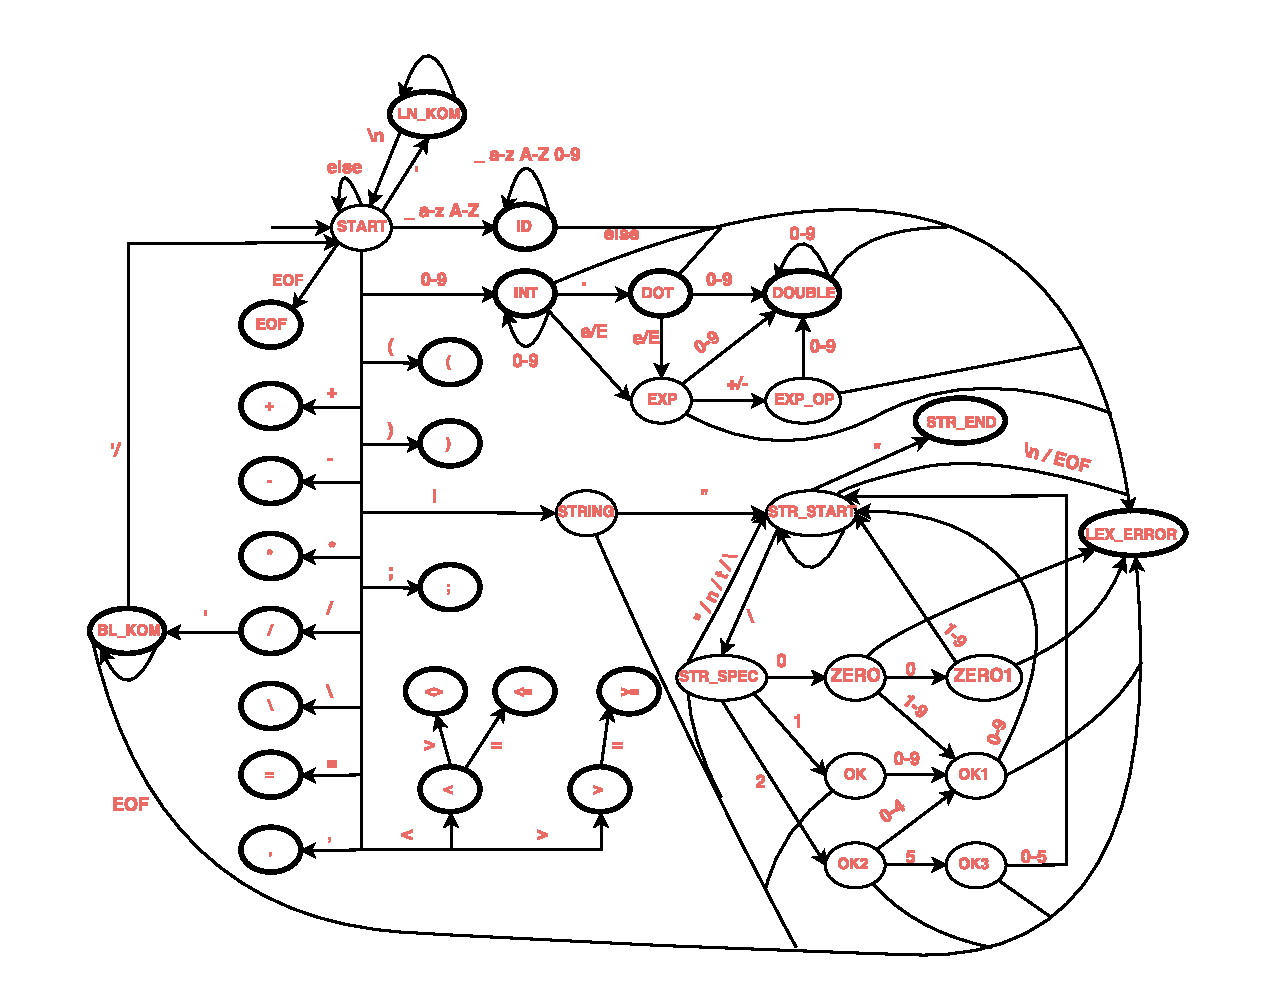
\includegraphics{scanner.eps}
}}
\caption{Konečný automat lexikálneho analyzátora}

\label{scanner}

\end{figure}

\end{document} 